\documentclass{article}
\usepackage[utf8]{inputenc}
\usepackage{minted}
\usepackage{amsmath}
\usepackage{tikz}
\usepackage{graphicx}
\usepackage{float}
\usepackage[document]{}
\usepackage[margin=1.5in]{geometry}

\title{An Exploration of PageRank and Similar Algorithms}
\author{Sidney Wang}
\date{\today}

\begin{document}

\maketitle

\section{Introduction}

PageRank is an algorithm used to generate a ranking of websites based on their relative importance. The algorithm has a number of practical applications, primarily in enabling search engines such as Google to deliver results for a given query. If a user of a search engine looks up a term, it's most helpful to them to provide trusted and popular sources as the top results, reducing the number of webpages the user must click through in order to find what they're looking for, and PageRank provides a way to determine the order in which sites should be displayed.

\section{The Basic Algorithm}

PageRank represents individual web pages as vertices in a graph. If web page A links to web page B, there will be a directed edge from A to B, indicating that B is reachable via A. Additionally, we weight the edges, such that the weight of the $A-B$ edge corresponds to the probability that the user navigates to page $B$ from $A$. If the user has multiple options, it's assumed that the user will pick one at random. This means the sum of all weights out of a vertex must be $1$.

To begin, every vertex is assigned an initial $PageRank$ value of $\frac{1}{n}$, where $n$ is the number of pages. The algorithm proceeds iteratively with the following steps performed every iteration until a converging $PageRank$ value for each vertex is found:

\begin{enumerate}
    \item Let $V$ be the in-neighbors of vertex $i$. Calculate $i$'s $PageRank$ as 
    \begin{equation}
        \sum\limits_{v \in V} \frac{PageRank(v)}{\text{out-degree of } v}
    \end{equation}
    \item Repeat for all vertices $i$ in the graph.
\end{enumerate}

After some number of iterations, the $PageRank$ for each vertex will not continue to change significantly, at which point the algorithm terminates.

\medskip
Let's examine one iteration on a simple example internet with pages A, B, and C, where page A links to page B, page B links to page C, and page C links to both A and B.

\begin{figure}[H]
    \begin{center}
    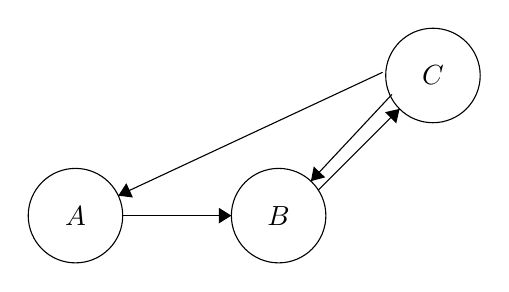
\begin{tikzpicture}[scale=0.2]
    \tikzstyle{every node}+=[inner sep=0pt]
    \draw [black] (22.3,-35.7) circle (3);
    \draw (22.3,-35.7) node {$A$};
    \draw [black] (35.2,-35.7) circle (3);
    \draw (35.2,-35.7) node {$B$};
    \draw [black] (45,-26.8) circle (3);
    \draw (45,-26.8) node {$C$};
    \draw [black] (25.3,-35.7) -- (32.2,-35.7);
    \fill [black] (32.2,-35.7) -- (31.4,-35.2) -- (31.4,-36.2);
    \draw [black] (37.7,-34.1) -- (42.88,-28.92);
    \fill [black] (42.88,-28.92) -- (41.96,-29.13) -- (42.67,-29.84);
    \draw [black] (42.4,-28) -- (37.25,-33.51);
    \fill [black] (37.25,-33.51) -- (38.16,-33.27) -- (37.43,-32.58);
    \draw [black] (41.8,-26.6) -- (25.02,-34.43);
    \fill [black] (25.02,-34.43) -- (25.95,-34.55) -- (25.53,-33.64);
    \end{tikzpicture}
    \end{center}
    \caption{Graph representation of the described internet}
    \label{fig:F1}
\end{figure}

\medskip

$n = 3$ so $PageRank(A) = PageRank(B) = PageRank(C) = \frac{1}{3}$ initially. For the next iteration, let's first examine $A$: it has one in-neighbor $C$ with degree 2 and $PageRank \frac{1}{3}$ so $A$'s new $PageRank$ is $\frac{1}{3} \cdot \frac{1}{2} = \frac{1}{6}$. $B$ however has two in-neighbors $A$ and $C$-- $A$ has out-degree 1 so it contributes $\frac{1}{3}$ towards $B$'s new $PageRank$. $B$ also has in-neighbor $C$ with degree $2$ so $C$ will contribute $\frac{1}{3} \cdot \frac{1}{2} = \frac{1}{6}$ towards $B$'s $PageRank$ for a total of $\frac{1}{3} + \frac{1}{6} = \frac{1}{2}$. Lastly, $C$ has in-neighbor $B$ with out-degree $1$ so $C$'s new $PageRank$ is $\frac{1}{3} \cdot 1 = \frac{1}{3}$.

\section{Issues with the Simple Algorithm}

A problem arises when we try to examine the arguably simplest multi-node internet. Consider a small internet where many pages exist independently with no links between them, but page $A$ links to page $B$:

\begin{figure}[H]
    \begin{center}
    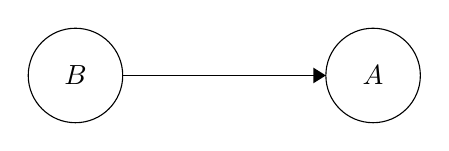
\begin{tikzpicture}[scale=0.2]
    \tikzstyle{every node}+=[inner sep=0pt]
    \draw [black] (22.3,-35.7) circle (3);
    \draw (22.3,-35.7) node {$B$};
    \draw [black] (41.2,-35.7) circle (3);
    \draw (41.2,-35.7) node {$A$};
    \draw [black] (25.3,-35.7) -- (38.2,-35.7);
    \fill [black] (38.2,-35.7) -- (37.4,-35.2) -- (37.4,-36.2);
    \end{tikzpicture}
    \end{center}
    \caption{Simple internet with $B$ linking to $A$}
    \label{fig:F2}
\end{figure}

Initially, $PageRank(B) = PageRank(A) = 0.5$ and after one iteration, $PageRank(B) = 0$ and $PageRank(A) = 0.5$. Notice that the sum of $PageRank$s is no longer $1$-- this becomes even more apparent after one further iteration, where we get $PageRank(B) = 0$ and $PageRank(A) = 0$. What happened?

Let's imagine a user browsing this internet. If they start at $B$ and click the link to $A$, there is nowhere further to go-- they're stuck at node $A$. For this reason, $A$ is a ``sink state''-- any user that navigates to $A$ at some point will be there forever. However, this is not realistic. If the contents of $A$ are boring or not satisfactory to the user, they will want to keep browsing and explore other random pages that are not linked directly to/from $B$ or $A$. PageRank solves this by introducing a ``damping factor'', or a small chance that instead of navigating to one of the available links from the current page, the user will pick a page at random next, in a different connected component. Expressed mathematically, $PageRank(i)$ is now defined as the following, where $d$ is the damping factor: 
\begin{equation}
    PageRank(i) = \frac{1-d}{n} + d\sum\limits_{v \in V} \frac{PageRank(v)}{\text{out-degree of } v}\
\end{equation}

The first term of the equation introduces the randomness that a user from any other page would jump to $i$ on the current iteration, and the second term remains unchanged except being scaled by a factor of $d$ to normalize the sum of all $PageRank$s to be $1$. 

Another way to think about the damping factor is to imagine adding ``ghost edges'' from every vertex to every other vertex, making the graph strongly connected. Each of these ghost edges should receive a weight of $\frac{1-d}{n}$, and any non-ghost edges (existing page links) going out of the vertex should have their existing weight scaled by a factor of $d$. 

\section{Implementing PageRank}
We can think of the adjacency matrix representation of our graph as a Markov matrix. Each column has sum $1$; since the next page the user visits must be some other page, and the total possibilities out of a page must sum to $1$. This leads to an alternate algorithm to performing the iterations stated previously-- instead of iterating until we reach a converging state, we can instead find the eigenvector associated with eigenvalue $1$ of the Markov matrix. I present a Julia implementation of this algorithm below (function \texttt{PageRank}).

\begin{minted}{julia}
using LinearAlgebra

# the probability that the user actually clicks on a link from the 
# current page instead of picking one at random
const DAMPING = 0.85
const EPSILON = 10^-5

# function to compare equality of two floats
function FloatEqual(x1::ComplexF64, x2::ComplexF64)
    return abs(x1 - x2) < EPSILON
end

# creates a map of each site to its index in the input
function MkIndexMap(sites::Vector{String}) 
    result = Dict{String, Int}()
    for i in 1:size(sites, 1)
        result[sites[i]] = i
    end
    return result
end

# this function takes in a list of websites, 
# and a list containing a list of outgoing links for each 
# website (adjacency list), returning an unweighted Adjacency Matrix 
# representation of the graph where 
# 1 = directed edge from col index -> row index and 0 = no edge
# links is assumed to contain [] for a specific vertex's adjacency list 
# if it has no out-neighbors
function MkGraph(sites::Vector{String}, links::Vector{Vector{Any}})
    # initialize an empty matrix of zeros
    result = zeros(size(sites, 1), size(sites, 1))
    indexMap = MkIndexMap(sites)
    for i in 1:size(links, 1)
        for j in 1:length(links[i])
            result[indexMap[links[i][j]], i] = 1
        end
    end
    return result
end    

# this function takes in an adjacency matrix and returns the weighted 
# transition matrix
# takes into account random jumps made by the user from page A to an 
# unlinked page
# invariant: every col in the returned matrix has sum 1
function MkTransition(graph::Matrix{Float64})
    len = size(graph, 1)
    # keep track of how many vertices are not immediate neighbors of v
    zeroes = zeros(len)
    # total probability of leaving a page is 1, so sum of each row should be 1
    for i in 1:len # column
        curr = sum(graph[:, i])
        for j in 1:len # row
            if graph[j, i] != 0 # prevent zero divisions if a vertex is isolated
                # normalize all values and account for randomness damping factor
                graph[j, i] /= curr
                graph[j, i] *= DAMPING
            else
                zeroes[i] += 1
            end
        end
    end
    # now add in the possibility to jump to a random page, for anything that's 
    # not linked
    # any "ghost edge" should have a weight of 
    # (1-damping) / (# of ghost edges out of v)
    # unless it's a lone vertex-- then visit any other page with equal 
    # probability
    for i in 1:len # column
        for j in 1:len # row
            if graph[j, i] == 0 && zeroes[i] != len
                graph[j, i] = (1-DAMPING) / zeroes[i]
            elseif graph[j, i] == 0
                # disconnected vertex, jump to a random page
                graph[j, i] = 1/len
            end
        end
    end
    return graph
end

# this function finds the index at which a particular value lives
function FindXIdx(list::Vector{ComplexF64}, x::ComplexF64)
    for i in 1:length(list)
        if FloatEqual(x, list[i])
            return i
        end
    end
end

# PageRank takes in a series of indexed websites, as well as a vector 
# containing vectors of pages that each indexed site links to
function PageRank(sites::Vector{String}, links::Vector{Vector{Any}})
    graph = MkGraph(sites, links)
    transition = MkTransition(graph)
    val, vec = eigen(transition)
    
    # identify the eigenvector associated w/ eigenvalue 1-- this is 
    # the solution
    idx = FindXIdx(convert(Vector{ComplexF64}, val), convert(ComplexF64, 1.0))
    soln = convert(Vector{Float64}, vec[:, idx])
    
    # soln contains the pageranks for each page
    # now, convert them to a ranked order
    enumerate = [(sites[i], soln[i]) for i in 1:length(sites)]
    final = sort(enumerate, by = x -> abs(x[2]), rev=true)
    return [final[i][1] for i in 1:length(final)]
end
\end{minted}

Note that the iterative version of the algorithm could be implemented by changing the implementation of \texttt{PageRank} to run iterations of the described algorithm instead of finding the eigenvector. This can be done by diagonalizing the Markov matrix and raising it to some converging power; alternatively, the Power method or other iterative algorithm to find the eigenvectors more efficiently can also be u sed. In practice, the creators of PageRank found that the number of iterations required of \texttt{PageRank} is small, even on a very large internet with hundreds of millions of vertices.

\section{The HITS Algorithm}
Hyperlink-Induced Topic Search, or HITS, is another algorithm used to rank webpages. It has some key differences from PageRank, namely that HITS takes into account the user's query and returns the most relevant pages, operates across a smaller subset of pages, and is calculated at the time of a query request due to its query-based nature. By contrast, PageRank is computed as the internet is indexed by some crawler that discovers new pages.

HITS, like PageRank, is an iterative algorithm. There is first a preprocessing step in which a ``root set'' is generated by selecting the pages most relevant to the user's query using some text-based searching algorithm. Then, a ``base set'' is generated that includes all out-neighbors of the root set and some in-neighbors of the root set. This is the graph upon which HITS will be run. 

Additionally, HITS uses the notion of an ``authority score'' and a ``hub score'' for each page instead of the singular $PageRank$ value. An authority can be thought of a trusted source linked to by many other pages, and a hub is some page that has compiled information, or has many links to other pages. Initialize each vertex's authority and hub scores to be 1.

The steps are as follows, repeated until converging values are found:

\begin{enumerate}
    \item Update each vertex's authority score to be the sum of hub scores of its in-neighbors.
    \item Update each vertex's hub score to be the sum of the authority scores of its out-neighbors.
    \item Normalize all values by dividing authority scores by the sum of squares of all authority scores, and repeat for hub scores.
\end{enumerate}

Let's examine an iteration of the same example from figure 1 earlier:
\begin{center}
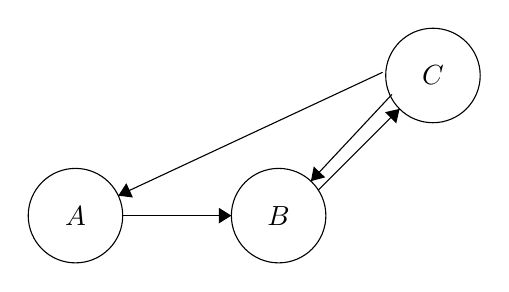
\begin{tikzpicture}[scale=0.2]
\tikzstyle{every node}+=[inner sep=0pt]
\draw [black] (22.3,-35.7) circle (3);
\draw (22.3,-35.7) node {$A$};
\draw [black] (35.2,-35.7) circle (3);
\draw (35.2,-35.7) node {$B$};
\draw [black] (45,-26.8) circle (3);
\draw (45,-26.8) node {$C$};
\draw [black] (25.3,-35.7) -- (32.2,-35.7);
\fill [black] (32.2,-35.7) -- (31.4,-35.2) -- (31.4,-36.2);
\draw [black] (37.7,-34.1) -- (42.88,-28.92);
\fill [black] (42.88,-28.92) -- (41.96,-29.13) -- (42.67,-29.84);
\draw [black] (42.4,-28) -- (37.25,-33.51);
\fill [black] (37.25,-33.51) -- (38.16,-33.27) -- (37.43,-32.58);
\draw [black] (41.8,-26.6) -- (25.02,-34.43);
\fill [black] (25.02,-34.43) -- (25.95,-34.55) -- (25.53,-33.64);
\end{tikzpicture}
\end{center}

$A$, $B$, $C$ all start with hub and authority scores of $1$. We first perform step 1, giving $A$, $B$, and $C$ new authority scores of $1, 2, 1$ respectively. Step 2 gives new hub scores of $2, 1, 3$ respectively. After normalizing, we get authority scores of $\frac{1}{2}, 1, \frac{1}{2}$ and hub scores of $\frac{2}{\sqrt{6}}, \frac{1}{\sqrt{6}}, \frac{3}{\sqrt{6}}$. 

\section{Implementing HITS}
The following is a Julia implementation of the previously described HITS algorithm (function \texttt{HITS}).

\begin{minted}{julia}
# decide whether to give more impact to pages that are hubs vs authorities
const HUB_WEIGHT = 1
const AUTHORITY_WEIGHT = 1

# builds a hash table of vertex -> all its in-neighbors
function MkInGraph(sites::Vector{String}, links::Vector{Vector{Any}})
    res = Dict{String, Set{String}}()
    for i in 1:length(sites)
        curr = links[i]
        for j in 1:length(curr)
            if !haskey(res, curr[j])
                res[curr[j]] = Set()
            end
            push!(res[curr[j]], sites[i])
        end
    end
    return res
end

# builds a hash table of vertex -> all its out-neighbors
function MkOutGraph(sites::Vector{String}, links::Vector{Vector{Any}})
    res = Dict{String, Set{String}}()
    for i in 1:length(sites)
        res[sites[i]] = Set(links[i])
    end
    return res
end

# sum of hub scores of x's in-neighbors
function GetAuthority(x::String, sites::Vector{String}, 
                      inGraph::Dict{String, Set{String}}, hub::Vector{Float64})
    total = 0
    for i in 1:length(sites)
        if sites[i] in inGraph[x]
            total += hub[i]
        end
    end
    return total
end

# sum of authority scores of out-neighbors
function GetHub(x::String, sites::Vector{String}, 
                outGraph::Dict{String, Set{String}}, authority::Vector{Float64})
    total = 0
    for i in 1:length(sites)
        if sites[i] in outGraph[x]
            total += authority[i]
        end
    end
    return total
end

function HITS(sites::Vector{String}, links::Vector{Vector{Any}})
    iNbors = MkInGraph(sites, links)
    oNbors = MkOutGraph(sites, links)
    # initialize all hub and authority values to be 1
    authority = normalize([1.0 for i in 1:length(sites)])
    hub = normalize([1.0 for i in 1:length(sites)])
    while true
        newAuthority = normalize([GetAuthority(sites[i], sites, iNbors, hub) 
        for i in 1:length(authority)])
        newHub = normalize([GetHub(sites[i], sites, oNbors, newAuthority) 
        for i in 1:length(hub)])
        if abs(sum(newAuthority) - sum(authority)) +
        abs(sum(newHub) - sum(hub)) < EPSILON
            authority = newAuthority
            hub = newHub
            break
        end 
        authority = newAuthority
        hub = newHub
    end
    # account for a page's importance by taking the sum of its 
    # scaled hub and authority scores
    final = [(AUTHORITY_WEIGHT * authority[i] + HUB_WEIGHT * hub[i], sites[i]) 
            for i in 1:length(sites)]
    sorted = sort(final, by = x -> abs(x[1]), rev=true)
    return [sorted[i][2] for i in 1:length(sites)]
end
\end{minted}

\section{PageRank vs HITS}
Let's compare the outputs of these two algorithms, with hub and authority having equal weight in HITS. Consider the following small internet (from Wikipedia):

\begin{figure}[H]
    \begin{center}
    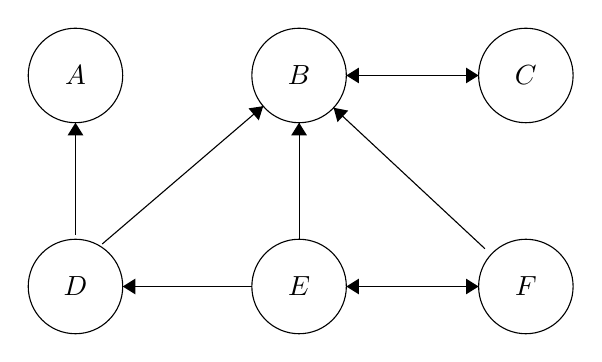
\begin{tikzpicture}[scale=0.2]
    \tikzstyle{every node}+=[inner sep=0pt]
    \draw [black] (15.8,-16.1) circle (3);
    \draw (15.8,-16.1) node {$A$};
    \draw [black] (30,-16.1) circle (3);
    \draw (30,-16.1) node {$B$};
    \draw [black] (44.4,-16.1) circle (3);
    \draw (44.4,-16.1) node {$C$};
    \draw [black] (15.8,-29.5) circle (3);
    \draw (15.8,-29.5) node {$D$};
    \draw [black] (30,-29.5) circle (3);
    \draw (30,-29.5) node {$E$};
    \draw [black] (44.4,-29.5) circle (3);
    \draw (44.4,-29.5) node {$F$};
    \draw [black] (15.8,-26.2) -- (15.8,-19.1);
    \fill [black] (15.8,-19.1) -- (15.3,-19.9) -- (16.3,-19.9);
    \draw [black] (33.2,-16.1) -- (41.4,-16.1);
    \fill [black] (41.4,-16.1) -- (40.6,-15.6) -- (40.6,-16.6);
    \draw [black] (41.4,-16.1) -- (33,-16.1);
    \fill [black] (33,-16.1) -- (33.8,-16.6) -- (33.8,-15.6);
    \draw [black] (41.8,-27.1) -- (32.19,-18.15);
    \fill [black] (32.19,-18.15) -- (32.44,-19.06) -- (33.12,-18.33);
    \draw [black] (30,-26.5) -- (30,-19.1);
    \fill [black] (30,-19.1) -- (29.5,-19.9) -- (30.5,-19.9);
    \draw [black] (27,-29.5) -- (18.8,-29.5);
    \fill [black] (18.8,-29.5) -- (19.6,-30) -- (19.6,-29);
    \draw [black] (17.5,-26.8) -- (27.72,-18.05);
    \fill [black] (27.72,-18.05) -- (26.79,-18.19) -- (27.44,-18.95);
    \draw [black] (33.3,-29.5) -- (41.4,-29.5);
    \fill [black] (41.4,-29.5) -- (40.6,-29) -- (40.6,-30);
    \draw [black] (41.4,-29.5) -- (33,-29.5);
    \fill [black] (33,-29.5) -- (33.8,-30) -- (33.8,-29);
    \end{tikzpicture}
    \end{center}
    \caption{Graph representation of the described internet}
    \label{fig:F1}
\end{figure}

According to the implementation, this gives the following arguments to \texttt{PageRank} and \texttt{HITS}:
\begin{minted}{julia}
sites = ["A", "B", "C", "D", "E", "F"]
links = [[], ["C"], ["B"], ["A", "B"], ["D", "B", "F"], ["E", "B"]]
\end{minted}

The two algorithms output the following rankings:
\begin{minted}{julia}
PageRank(sites, links)
> ["B", "C", "E", "A", "D", "F"]
HITS(sites, links)
> ["B", "E", "D", "F", "C", "A"]
\end{minted}

Intuitively, we expect $B$ to be at the top of the ranking, since it has by far the most in/out-neighbors, but the two algorithms don't seem to agree on the rankings beyond that. One reason for this is that in this implementation of HITS it's possible to decide how important a hub vs an authority is, while PageRank places more value on the neighbors of pages that have fewer links. That is, anyone that is a neighbor of a large hub will not have a large $PageRank$ value due to its in-neighbor's edge weight being very small. HITS also doesn't account for the fact that authority links should be more likely to be trusted; if $A$ is a large authority and $B$ is its only out-neighbor, $B$ will not be valued highly as an authority itself since its authority score depends on $B$'s hub score, which is dependent on $B$'s in-neighbors' authority scores. Additionally, HITS does not account for the damping factor and is more similar to a random walk and is normally run on a subset of a larger internet.

\section{Further Exploration}
As it turns out, the Internet is very big. This means that although the creators of PageRank have concluded that the algorithm converges quickly on very large datasets, there remains the question of how to store this data and manipulate it. One way is to scale out, or add more computation capable nodes, cleverly divide the problem into slices, and give each node a slice to work on. Then, putting together each node's answer gives the final answer. This is more realistic than buying an extremely high-powered machine with enormous storage (scaling up); doing so would not only be very expensive, but once the storage fills up (the Internet only gets bigger), you are stuck. Additionally, if the machine crashes, or the power goes out, or any other failure occurs, it is difficult to keep a backup copy of the data.

MapReduce (also developed by Google) is a great way to divide the work among nodes and aggregate their computations. Generally, no single node is capable of storing the entire dataset an operation is to be performed on, but each is happy to store some subsection of the data. Mapreduce generally works as follows:
\begin{enumerate}
    \item \textbf{Map:} Each node applies a \texttt{map} function to map all inputs to (key, value) pairs.
    \item \textbf{Shuffle:} All pairs with the same key are given to the same node.
    \item \textbf{Reduce:} The node reduces all pairs with the same key in parallel by applying some reduction function of type \texttt{((key, value), (key, value)) -> output}.
\end{enumerate}

The output from reduce can then be fed into another round of MapReduce. 

Represent the graph as an adjacency list. (key, value) pairs are (a vertex, its neighbors). Give each node some subset of the vertices to be responsible for.

For the map: for each vertex, calculate the outgoing edge weight and alert the neighbors of this value.

For reduce, each node should reduce by summing the incoming weights (in-neighbors), which can be parallelized for each unique vertex. This is now the new $PageRank$ value for the next iteration.

\medskip
MapReduce is not ideal for computing most iterative algorithms, but PageRank converges in very few iterations, making it a suitable candidate. Using MapReduce techniques is one way to eliminate one of the largest issues with storing data. In practice, the web is always expanding and the next iteration of MapReduce cannot be run until the previous one terminates. However, since significant parallelism is introduced, the time to compute one iteration is efficient and any newly discovered links can be added the following iteration.

\section{Things I Learned}

Through researching for this project, I learned about some elegant algorithms that uses the math we've seen in class to a real-world application. It's possible to understand these algorithms with no real matrices background, but understanding the relatively uncomplicated math motivating the algorithm leads to a much more satisfying and beautiful understanding. It's fascinating to me to think about the impact a relatively simple, very understandable algorithm has had on how we think about searching the internet, as well as the company that it kickstarted (Google).

This project also gave me a new appreciation into the use of matrices as a data structure, just like graphs, heaps, priority queues, and others. Matrices are a tool for abstracting a real problem into a form upon which we can apply familiar CS/math techniques, and learning about PageRank and HITS made me really realize that for the first time.

Lastly, exploring some ways PageRank might be optimized to run on a sizeable internet was an interesting way for me to connect what I learned in this project to other interests. One of the best ways to speed something up is to scale out, but making efficient use of resources is always challenging in Distributed Systems problems. I was curious whether or not MapReduce and related techniques could be applied given that PageRank converges in few iterations and the dataset is very large (billions of vertices and edges). Learning how the two algorithms fit together was very interesting, as was seeing the two flavors of CS come together-- one more concerned with practicality, and the other of a more algorithmic/theoretical type.

\begin{thebibliography}{9}
\bibitem{harvard}
Harvard OpenCourseWare, \emph{PageRank}, https://cs50.harvard.edu/ai/2020/projects/2/pagerank/.

\bibitem{julia}
Julia Programming Language, \emph{Julia 1.8 Documentation}, https://docs.julialang.org/en/v1/.

\bibitem{medium}
Kabbani Taylan, \emph{PageRank on MapReduce}, https://medium.com/swlh/pagerank-on-mapreduce-55bcb76d1c99.

\bibitem{overleaf}
Overleaf, \emph{Documentation}, https://www.overleaf.com/learn.

\bibitem{original paper} 
Page, Lawrence and Brin, Sergey, \emph{The PageRank Citation Ranking:
Bringing Order to the Web}, http://ilpubs.stanford.edu:8090/422/1/1999-66.pdf.

\bibitem{utah}
Phillips, Jeff, \emph{PageRank on MapReduce}, 
https://www.cs.utah.edu/~jeffp/teaching/cs5140-S15/cs5140/L24-MR+PR.pdf.

\bibitem{cornell}
Tanase, Raluca and Radu, Remus, \emph{HITS Algorithm - Hubs and Authorities on the Internet}, http://pi.math.cornell.edu/mec/Winter2009/RalucaRemus/Lecture4/lecture4.html.

\bibitem{fsm}
Wallace, Evan, \emph{Finite State Machine Designer}, https://madebyevan.com/fsm/.

\bibitem{wikipedia hits}
Wikipedia, \emph{HITS algorithm}, https://en.wikipedia.org/wiki/HITS\_algorithm.

\bibitem{wikipedia mapreduce}
Wikipedia, \emph{MapReduce}, https://en.wikipedia.org/wiki/MapReduce.

\bibitem{wikipedia}
Wikipedia, \emph{PageRank}, https://en.wikipedia.org/wiki/PageRank.

\end{thebibliography}

\end{document}